\graphicspath{{chapters/images/02/}}

\chapter{Working with transcriptomics}

  \section{Measuring RNAs and proteins}
    There are several ways to measure proteins (western blot, ELISA, northern blot, enzymatic assay) and RNAs (microarray, RT-PCR, RNA-Seq). Protein and mRNA levels often do not correlate (or only loosely); for this reason, studying directly the protein levels would be the best option. Yet again, due to the fact that there are no high throughput methods for absolute protein quantification, no genome-wide protein arrays and the fact that protein sequencing is difficult, more often then not mRNA levels are still used. The two main approaches for transcript measurement are DNA microarrays and RNA-seq. 

  \section{DNA microarrays}
    For microarray protocol see previous chapter.
    % TODO Add reference

    \subsection{Most common microarrays}
      DNA microarrays are the older technology for RNA quantification (started in the early '90s). Early microarrays were glass slides with probes spotted by the individual laboratories, then companies started producing more refined versions. One of the most used devices is the \textbf{Affymetrix GeneChip}, capable of analyzing all the genes of an organism (available for different species), with multiple oligonucleotide-probes per transcript, with control mismatch sequences. It allows to analyze one sample at a time and to obtain an absolute quantification of the transcript levels (more or less). Another common technology is \textbf{Illumina BeadChip}, in which the probes are spotted on beads placed in wells. Compared to Affymetrix GeneChip, Illumina BeadChip has higher throughput and allows the use of two fluorescent molecules at the same time.
    
    \subsection{Microarrays advantages}
      Microarrays allow to quantify not only mRNAs, but also miRNAs, SNPs and others. They allow to study all the genes in the genome, including the splicing variants, and they are reliable for gene expression quantifications (and comparative analysis). They are cost effective and easy to analyze, thanks to the bioinformatics resources that are now available. Microarrays give direct (non-absolute) quantification of the mRNA.

	  \begin{figure}[ht]
	  \caption{}
	  \centering
	  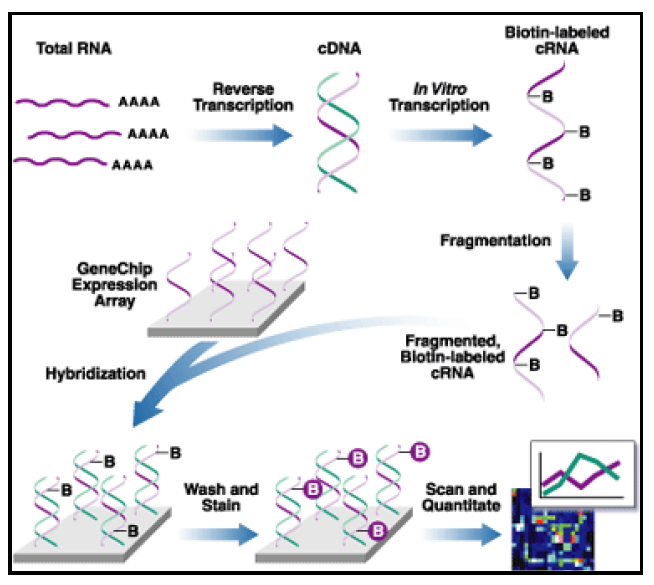
\includegraphics[width=0.6\textwidth]{microarrays}
	  \end{figure}

    \subsection{Error sources in microarrays}
      There are several possible sources of error when working with microarrays:
      \begin{itemize}
        \item RNA contamination during extraction 
        \item Poor quality, insufficient extraction or degradation of RNA
        \item Bias in which molecules are transcribed during retro transcription
        \item Bias in ligation of the fluorescent protein reporter
        \item Cross hybridization, meaning the aspecific binding to the wrong probe (especially if the sequence is long)
        \item Aspecific fluorescence and in general background noise
        \item Scanning errors during image acquisition
      \end{itemize}

	  \begin{figure}[ht]
	  \caption{}
	  \centering
	  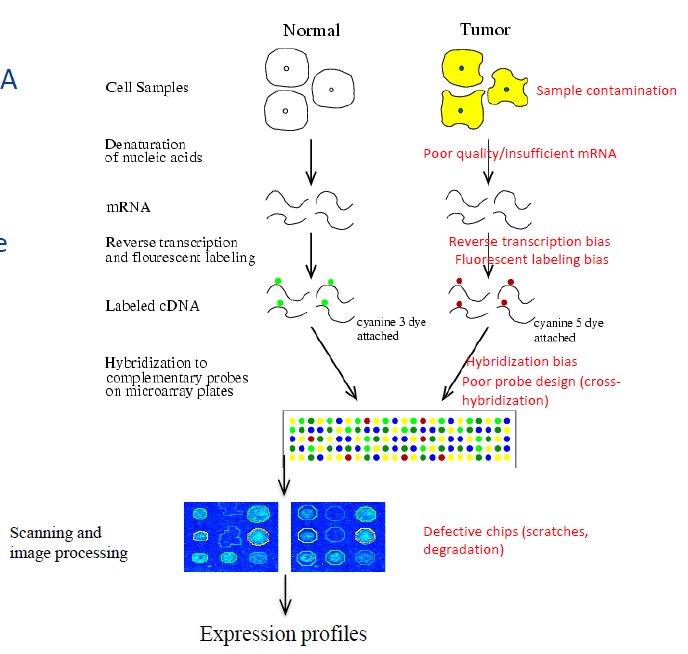
\includegraphics[width=0.6\textwidth]{ProblemsMicarrays}
	  \end{figure}

	\subsection{Noise handling and normalization in microarrays}
      Some methods exist to reduce the noise (error). For instance, the Affymetrix GeneChip uses two probes for each transcript, one with perfect match and one with a single \textbf{mismatch}; if you subtract the mismatch fluorescent from the perfect match one, you remove some of the fluorescence signal due to aspecific interactions (it is not the most efficient correction). Moreover Affimetrix GeneChips come with quality control checks data. 
      Another way to remove noise is \textbf{Robust Multi-array Average (RMA)} which is an algorithm that takes into account the fluorescence levels of the entire chip and applies a correction. 
      \textbf{Spy probes} are basically control probes, meaning that they should not show any sign of fluorescence; these probes are useful to detect contaminations (for instance you can use mouse-RNA probes on human-RNA chips).

      In order to obtain an absolute quantification of the transcript levels, other steps are required in addition to noise correction; these steps are generally referred to as normalization. These steps make use of statistical tools, control genes and others to correct for chip, probe, spatial, intra and inter chip variation.

    \subsection{Other problems with microarrays}
      Further problems regarding microarrays can be found:
      \begin{itemize}
		\item A certain transcription level (detection limit) is required to have a signal
		\item To quantify a transcript, a probe for it must be present on the chip (therefore you cannot study unknow transcripts)
		\item Most chips cannot differentiate splicing variants well (even though there are some chips that try), since usually the match is checked for a subset of the sequence 
		\item Chips cannot differentiate RNA synthesis and degradation
		\item Chips do not provide information on post translational events
		\item The bioinformatic analysis may be difficult
      \end{itemize}

    \subsection{Microarray data processing}
      An Affymetrix GenexChip generates several type of files:
      \begin{itemize}
      	\item DAT (image file)
      	\item CEL (raw data file)
      	\item CDF (chip definition file)
      \end{itemize}
	  All platforms have different data formats, which can complicate the analysis.  
      \textbf{Bioconductor} is a open source software project for the analysis and comprehension of genomic data. It provides a wide range of powerful statistical and graphical tools.

	  Microarray data can be found in repositories, such as \textbf{Array express} (UK), \textbf{Gene Expression Omnibus}(founded by NIH, USA), CIBEX (JP). Notice that Array express and GEO contain non-overlapping data. \textbf{Recount3} has a smaller number of datasets, most of which already in GEO, but these datasets have already been partially processed. Other databases can be used for annotation purposes, such as NetAffx, Ensembl, TIGR and Stanford. 

      There are some microarray data standards, namely:
      \begin{itemize}
      	\item \textbf{MIAME} (Minimum annotation about a microarray experiment); this entails a comprehensive description of the experiment, therefore allowing replicates of chips, samples, treatments and settings and facilitating data comparison. It is required for most recent publications.
      	\item \textbf{MAGE-ML} (Microarray gene expression markup language). It describes both the experiment (MIAME) and the data. Tools are available for processing this format.
      \end{itemize}


  \section{RNA-Seq}

	RNA-Seq is a more recent way of measuring gene expression levels which uses next generation sequencing techniques. The idea is that, by sequencing each molecule in the sample, you are able to obtain an absolute quantification.
    
    \subsection{RNA-Seq workflow}
      A \textbf{whole transcriptome shotgun sequencing} approach is used. The general workflow can be described as follows:
      \begin{itemize}
        \item The whole RNA content of the sample is broken into fragments using restriction enzymes; this is repeated for multiple samples with different restriction enzymes in order to have different breaking points (and thus facilitating following steps since it increases the amount of overlapping segments).
        \item RT-PCR is performed in order to obtain cDNA from all fragments. Each cDNA fragment is sequenced and the results are called \textbf{raw reads}, which are store in a fastQ file, which is a text-file where each row is a sequence (produced by Illumina sequencing machines).
        \item Quality control is performed on the reads (sequence quality, GC content, presence of adaptors, overrepresented K-mers, duplicated reads). After quality control and adaptor sequence trimming you obtain the \textbf{reads}.
        \item The reads are then re-assembled and mapped against a reference sequence (genome for splicing information, transcriptome for faster computation) in order to obtain the original sequences present in the sample. This step requires a computer with a lot of ram and storage, way more than the average laptop; cloud computing is a way to solve this problem. The output is generally stored in a BAM file, which is a text-file with each read and next to it the coordinates with reference to the genome.
        \item After mapping, the number of reads for each sequence is computed; those integer numbers are called \textbf{raw counts} and are stored in a count matrix where each row is a gene, and each column a sample, each cell is the number of counts for that gene in that sample. The database recount3 provides count matrices from some RNA-Seq experiments.  
        \item Pre-processing refers to a series of steps used to remove bias and normalize your data (inter and intrea sample normalization, normalize for gene lenght, normalize for number of reads per sample); the output are the \textbf{counts}, 
        \item Counts can be used for several types of analyses, such as differential expression analysis, functional analysis, network-based enrichment analysis.
      \end{itemize}
      %TODO Add image
    
    \subsection{RNA-Seq data normalization}
      Several normalization algorithms are available, both for within-sample normalization and for between-sample normalization (for instance if you want to perform t-test on differential gene expression); some of them are shown in the tables below.
      %TODO Add reference images
      Notice that sometimes the order of the normalization steps actually matters (TPM is slightly better than RPKM for instance).
